\documentclass[a4paper]{article}

\usepackage{xcolor}
\usepackage{fancyheadings}
\usepackage{graphicx}


\newcommand{\todo}[1]{\textcolor{red}{[#1]}}
\lhead{Open Universiteit}
\chead{IM0102, Design patterns}
\rhead{Eindopdracht}

\begin{document}
\pagestyle{fancy}

\section*{Studentgegevens}
\begin{description}
	\item [Cursuscode] IM0102
	\item Scenario 6: Meerdere slidesets
	\item [Naam] Gerwin van Dijken
	\item [Studentnummer] \todo{invullen}
	\item [Naam] Ewoud Westerbaan
	\item [Studentnummer] 852069942
\end{description}

\section*{Aanpak}
\todo{<Geef aan hoe jullie de opdracht hebben aangepakt en wie wat heeft gedaan, maximaal 1 A-4. Geef expliciet aandacht aan de volgorde van activiteiten>}
Uit leereenheid 3 de huidige beschrijving gehaald
Deze uitgebreid met de concepten uit de scenario beschrijving



\section{Probleemanalyse}
\subsection{Dingen}
\begin{description}
\item[Presentatie] is de weergave van gespecificeerde slides in een vaste volgorde. Slides kunnen meerdere keren voorkomen. Een presentatie bevat een titel. Deze is altijd zichtbaar tijdens de weergave van de presentatie. In het programma kunnen meerdere presentaties beschikbaar zijn.
\item[Slide] is de weergave van een pagina op het scherm. Een slide heeft een titel, een nummer, slide items en heeft een bepaalde oppervlakte.
\item[Slide item] is een element op een slide. Slide items worden onder elkaar getoond en is van een bepaalde type.
Een slide item wordt in een stijl te gepresenteerd.
\item[Stijl] is een vorm van weergave van een slide item in termen van horizontale uitlijning, lettertype, kleur, en lettertypegrootte.
\end{description}

\subsection{Regels}
\begin{description}
\item[Presentatie] bepaalt de volgorde van de slides.
\item[Slide item] bepaalt de stijl van de weergave.
\item[Stijl] bepaalt doe een slide item wordt weergegeven. 
\end{description}

\subsection{Verantwoordelijkheden}
\begin{description}
\item[Presentatie] is verantwoordelijk voor de correcte volgorde van de slides en het beschikbaar stellen hiervan. 
\item[Slide] kan zijn titel tonen en de slide items schalen en onder elkaar laten tekenen.
\item[Slide item] kan zichzelf tekenen.
\end{description}
Overige verantwoordelijkheden die in de applicatie verwerkt moet worden:
\begin{description}
\item[Inlezen] van een XML bestand waarin de presentaties opgeslagen zijn. Uit dit bestand moet de slides verzameling en presentaties opgebouwd worden.
\item[Laten zien] van een gebruikers interface. Een gebruiker moet een presentatie kunnen kiezen, de presentaties kunnen bekijken en er doorheen kunnen navigeren.
\end{description}

\subsection{Aannames}
\todo{Hoe gaan we nu om met bestanden waar geen slidesequence in staat?}.

\section{Ontwerp}
\begin{description}
\item[Presenter] is verantwoordelijk voor de omgang van meerdere presentaties en het bijhouden wat de actieve presentatie is. Het biedt afnemers de mogelijkheid om een presentatie te kiezen.
\item[Presentation] is verantwoordelijk voor de correcte volgorde van de slides, het beschikbaar stellen hiervan en afnemers laten weten dat de slide beschikbaar is. Het biedt mogelijkheden om door slides te navigeren.
\item[Slide] is verantwoordelijk voor het tekenen van zichzelf.
\item[SlideItem] Zorg dragen voor het tekenen van items.
\item[Item] is verantwoordelijk voor het tekenen van zichzelf.
\item[Loader] Laden van presentaties.
\end{description}
Om te kunnen reageren op wijzigingen van het model, zijn er twee observers gespecificeerd:
\begin{description}
\item[PresentationObserver] verantwoordelijk voor het reageren op wijziging van de presentatie. Bijvoorbeeld het veranderen van een presentatie.
\item[SlideObserver] verantwoordelijk voor reageren op het wijzigen van de aangeboden slide (dat er een andere slide ter beschikking wordt gesteld).
\end{description}

\section{Keuzen}
\begin{description}
\item[Model-View-Controller] als architectuur ontwerp. Het model is verantwoordelijk voor het kenbaar maken van wijzigingen. Dit wordt gedaan door het Observer patroon twee keer toe te passen.
\item[SlideObserver] Voor het kenbaar maken dat een andere slide getoond moet worden, hebben we gekozen voor het observer pattern. De reden is dat in de toekomst mogelijk andere observers ook acties moeten uitvoeren op het moment dat een andere slide getoond wordt. Te denken is aan een presentatorscherm waar opmerkingen op getoond worden. Aan de Observers wordt de nieuw actieve Slide gegeven.
\begin{itemize}
\item Subject: Presenter
\item Observer: SlideObserver
\end{itemize}
\item[PresentationObserver] In deze versie van de applicatie is de toevoeging dat er met andere presentaties (volgorde van slides) gewerkt moet kunnen worden. Om andere objecten te laten weten dat de presentatie gewijzigd is, hebben we een PresentationObserver gemaakt. Aan de observers wordt de nieuw actieve Presentation gegeven.
\begin{itemize}
\item Subject: Presenter
\item Observer: PresentationObserver
\end{itemize}
\item[Iterator] Voor het aanbieden van slides aan de afnemer hebben we gekozen voor een (soort van) iterator patroon. De afnemers, alle SlideObservers moet beschikking hebben over de objecten (Slides). Toch is dit geen zuivere Iterator in die zin dat de afnemende objecten niet vragen aan de Aggregate (Presenter) om een specifieke Iterator (Presentation) en hier methodes op aanroepen. In deze implementatie houdt de aggregate (de Presenter in ons geval) zelf bij wat de actieve iterator is, dit is immers zijn verantwoordelijkheid. Een actie als next() en previous() zal de Presenter op de actieve Iterator (Presentation) doen. Omdat de Presenter de Presentations gebruikt, creeërt de Presenter deze Presentations dus niet (in tegenstelling tot een klassieke iterator patroon), maar wordt dit gedaan door een factory (scheiding van creatie en gebruik).
\begin{itemize}
\item Aggregator: Presenter
\item Iterator: Presentation
\item ConcreteAggregator: PresentationManager
\item ConcreteIterator: SlideSequence
\end{itemize}

\item[Strategy] De SlideItem heeft een Item en een Style. De SlideItem geeft de Style aan de Item om deze zichzelf te tekenen. De implementatie van het tekenen met een gegeven stijl kan anders zijn voor de verschillende type items.
\begin{itemize}
\item Strategy: Item
\item ConcreteStrategies: TextItem, BitmapItem
\item Context: SlideItem
\end{itemize}

\end{description}
\subsection{Toekomstige veranderingen}
\begin{description}
\item[Bepaalde delen laten zien] Het laten zien van bepaalde delen van een slide is gegeven als een mogelijke verandering. Dit is te implementeren door een nieuwe concrete klasse te definiëren die de Slide interface implementeerd. Door deze klasse een associatie te gaven naar de SlideDeckSlide kan de klasse de SlideItems benaderen. De implementatie van de draw() methode hoeft dan alleen deze specifieke SlideItems op te halen. De SlideFactory zal wel aangepast moeten worden om de nieuwe implementatie als Slide terug te kunnen geven. Zo ook de Reader objecten omdat dit ook een wijziging is in hoe de presentaties zijn opgeslagen. Zie Figure \ref{fig:mogelijkeuitbreiding}, de concrete klasse is hier PresentationSlide genoemd.
\begin{figure}[htbp]
\caption{Mogelijke uitbreiding}
\centering
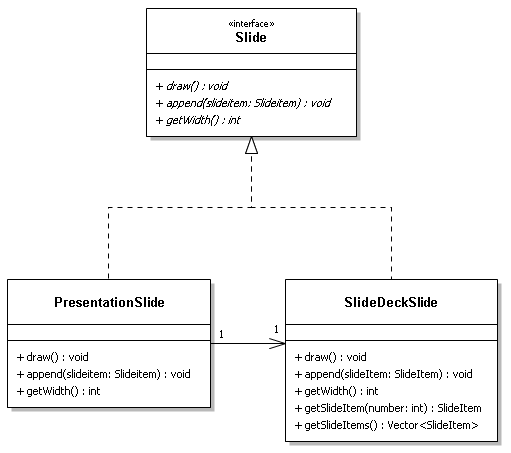
\includegraphics[width=0.75\textwidth]{MogelijkeUitbreiding.PNG}
\label{fig:mogelijkeuitbreiding}
\end{figure}
\item[Meerdere views] Zoals al aangegeven bij de observer pattern, is het mogelijk om bijvoorbeeld een aparte presentator view te maken waar opmerkingen op te zien zijn.
\item[Andere type items] Het is mogelijk om andere type items te tonen op een slide, door een nieuwe concrete klasse te maken die de Item interface implementeerd.
\end{description}


\section{Sourcecode}
De sourcecode bevat commentaar en beschrijvende tekst in JavaDoc formaat.

\end{document}
